\documentclass[a4paper,11pt]{article}
\usepackage{amsmath}
\usepackage{amssymb}
\usepackage{fullpage}
\usepackage{rotating}
\usepackage{tikz} \usetikzlibrary{trees}

\newcommand{\AnyCond}[1]{\text{Any}(#1)}
\newcommand{\BoundedCond}[1]{\text{Bounded}(#1)}
\newcommand{\Constraint}[1]{\textsc{#1}}
\newcommand{\DepProps}{\textit{DepProps}}
\newcommand{\Distinct}{\Constraint{Distinct}}
\newcommand{\Element}{\Constraint{Element}}
\newcommand{\Failed}{\text{Failed}}
\newcommand{\FailedCond}[1]{\text{Failed}(#1)}
\newcommand{\FixedCond}[1]{\text{Fixed}(#1)}
\newcommand{\Fixpoint}{\text{AtFixpt}}
\newcommand{\NoneCond}[1]{\text{None}(#1)}
\newcommand{\Gecode}{\textit{Gecode}}
\newcommand{\GIST}{\textit{GIST}}
\newcommand{\Propagate}{\text{Propagate}}
\newcommand{\PropConds}[1]{\text{PropConds}(#1)}
\newcommand{\Sequence}[1]{\left[#1\right]}
\newcommand{\Set}[1]{\left\{#1\right\}}
\newcommand{\Subsumed}{\text{Subsumed}}
\newcommand{\Tuple}[1]{\left\langle#1\right\rangle}
\newcommand{\Unknown}{\text{Unknown}}

%Min commandon
\newcommand{\Tdots}{\, .\, .\,}

%\pagestyle{empty}

\renewcommand{\thesubsection}{\Alph{subsection}}
\renewcommand{\thesubsubsection}{\Alph{subsection}.\alph{subsubsection}}

\title{\textbf{Low-Level Parallel Programming \\
    Uppsala University -- Spring 2015 \\
    Report for Lab~1
    by Team~21  % replace t by your team number
  }
}

\author{Markus Palacios, Jonathan Sharyari, Peng Sun} % replace by your name(s)

%\date{Month Day, Year}
\date{\today}


\begin{document}
\maketitle

\section{Questions}
\begin{description}
    \item[A] \textbf{What kind of parallelism is exposed with your code refactorization?}
 \hfill \\ 
As in lab 1, we are utilizing data parallelism.
    \item[B] \textbf{Give a short summary of similarities between SIMD and CUDA} \hfill

Both techniques are efficient for data parallelism; they are able to execute the same instructions on multiple sets of data in parallel.
    
    \item[C] \textbf{Which parallelization has been most beneficial in these two labs? Support your case using plotted timing measurements} \hfill \\
The answer depends on the size of the input. For really small problems a straight forward serial version will be faster (we have not generated a graph showing this), but the gains of parallelism increase with the size of the problem. We compared the techniques for an instance with 2048 agents and a large instance with 480000 agents. We used 4 processes for openMP and 2 processes for pthreads, as these were the settings yielding the best results in lab1 for the two techniques.

The techniques showed that SIMD gave the by far best speedup for the moderate scenario (2048 agents), iwhereas CUDA performed notabely worse than the serial version, this can be seen in the figure \ref{graph1}. For the large scenario, the speedup of CUDA was increased up to the point that it became the fastest technique, followed again by SIMD, see figure \ref{graph2}. This shows that the a large number of parallel calculations are needed in order for CUDA to really pay off.

We might note that openMP and Pthreads are far from unnecessary for solving this problem; there is nothing preventing us to utilize these techniques in combination with SIMD techniques, giving yet better speedups. Although doing so would be trivial, this is not the approach taken when generating the above graphs.

We must also note that there are other differences between the techniques than their underlying structures: In order to fully utilize data parallelism with SIMD and CUDA, we factored out a number of functions. We expect that the \texttt{go} and \texttt{whereToGo} functions used by SIMD and CUDA are more efficient per se.

    \item[D] \textbf{What kind of code transformations were required for this lab, and why were they
needed?} \hfill \\in $ped_agent.h$, the agent's x,y and z-values were stored in a struct. This made it hard for us to utilize parallelization in SIMD, as we'd always have to write each value to an array. This is a classical problem when attempting to exploit data parallelism -- a struct of arrays is preferable over an array of structs, in order to get good cache locality and avoid false sharing. We chose to instead instantiate arrays that hold each of the agents' x, y and z values together with their waypoints and other information needed to calculate the trajectory of the agents. In short, each agent stores not their values, but pointers to where their values are stored in a struct. This enabled us to implement the SIMD and CUDA versions with minimal changes to the already existing infrastructure utilized by openMP and Pthreards.

As mentioned above, neither CUDA nor SIMD uses the pre-existent functions Go() and whereToGo(), and instead calculates these values by themselves.

    \item[E] \textbf{Compare the effort required for each of the four parallelization techniques. Would
it have made a difference if you had to build the program from scratch, instead
of using given code?} \hfill \\ Yes. Since we've been forced to make major changes to how the program is implemented, it would have been easier to simply adapt the algorithm to fit our parallelization techniques instead of rewriting the existing one. 
\end{description}

\section{How to run}
Without an argument specifying the type of parallelism, the serial version is used, whereas --pthreads, --openmp, --vector and --cuda activate pthreads, openmp, vector and cuda respectively (in case both are set, the last occurance will be dominating). The number of threads can in both cases be set by --np X. The value of X is ignored in the serial case. Timing mode is enabled by adding --timing-mode to the commandline. An xml-formatted scenario may be specified by writing the name of the xml file in the command-line, if none is mentioned, "scenario.xml" will be used.
\begin{description}
    \item[Serial] ./demo
    \item[OpenMP] ./demo --openmp
    \item[Pthreads] ./demo --pthreads --np 4
    \item[Vector] ./demo --timing-mode --vector
    \item[CUDA] ./demo --cuda hugeScenario.xml
\end{description}
   
\subsection{Experiments}
Our experiments were run under Ubuntu Linux ~14.04 (64~bit) on an
Intel Core~i3~550 of 3.2~GHz with an 4~MB L2 cache and a 4~GB RAM.



\section*{Intellectual Property}
We certify that this report is solely produced by us, except where
explicitly stated otherwise and clearly referenced, and that we can
individually explain any part of it at the moment of submitting this
report.



\begin{figure}[h!]
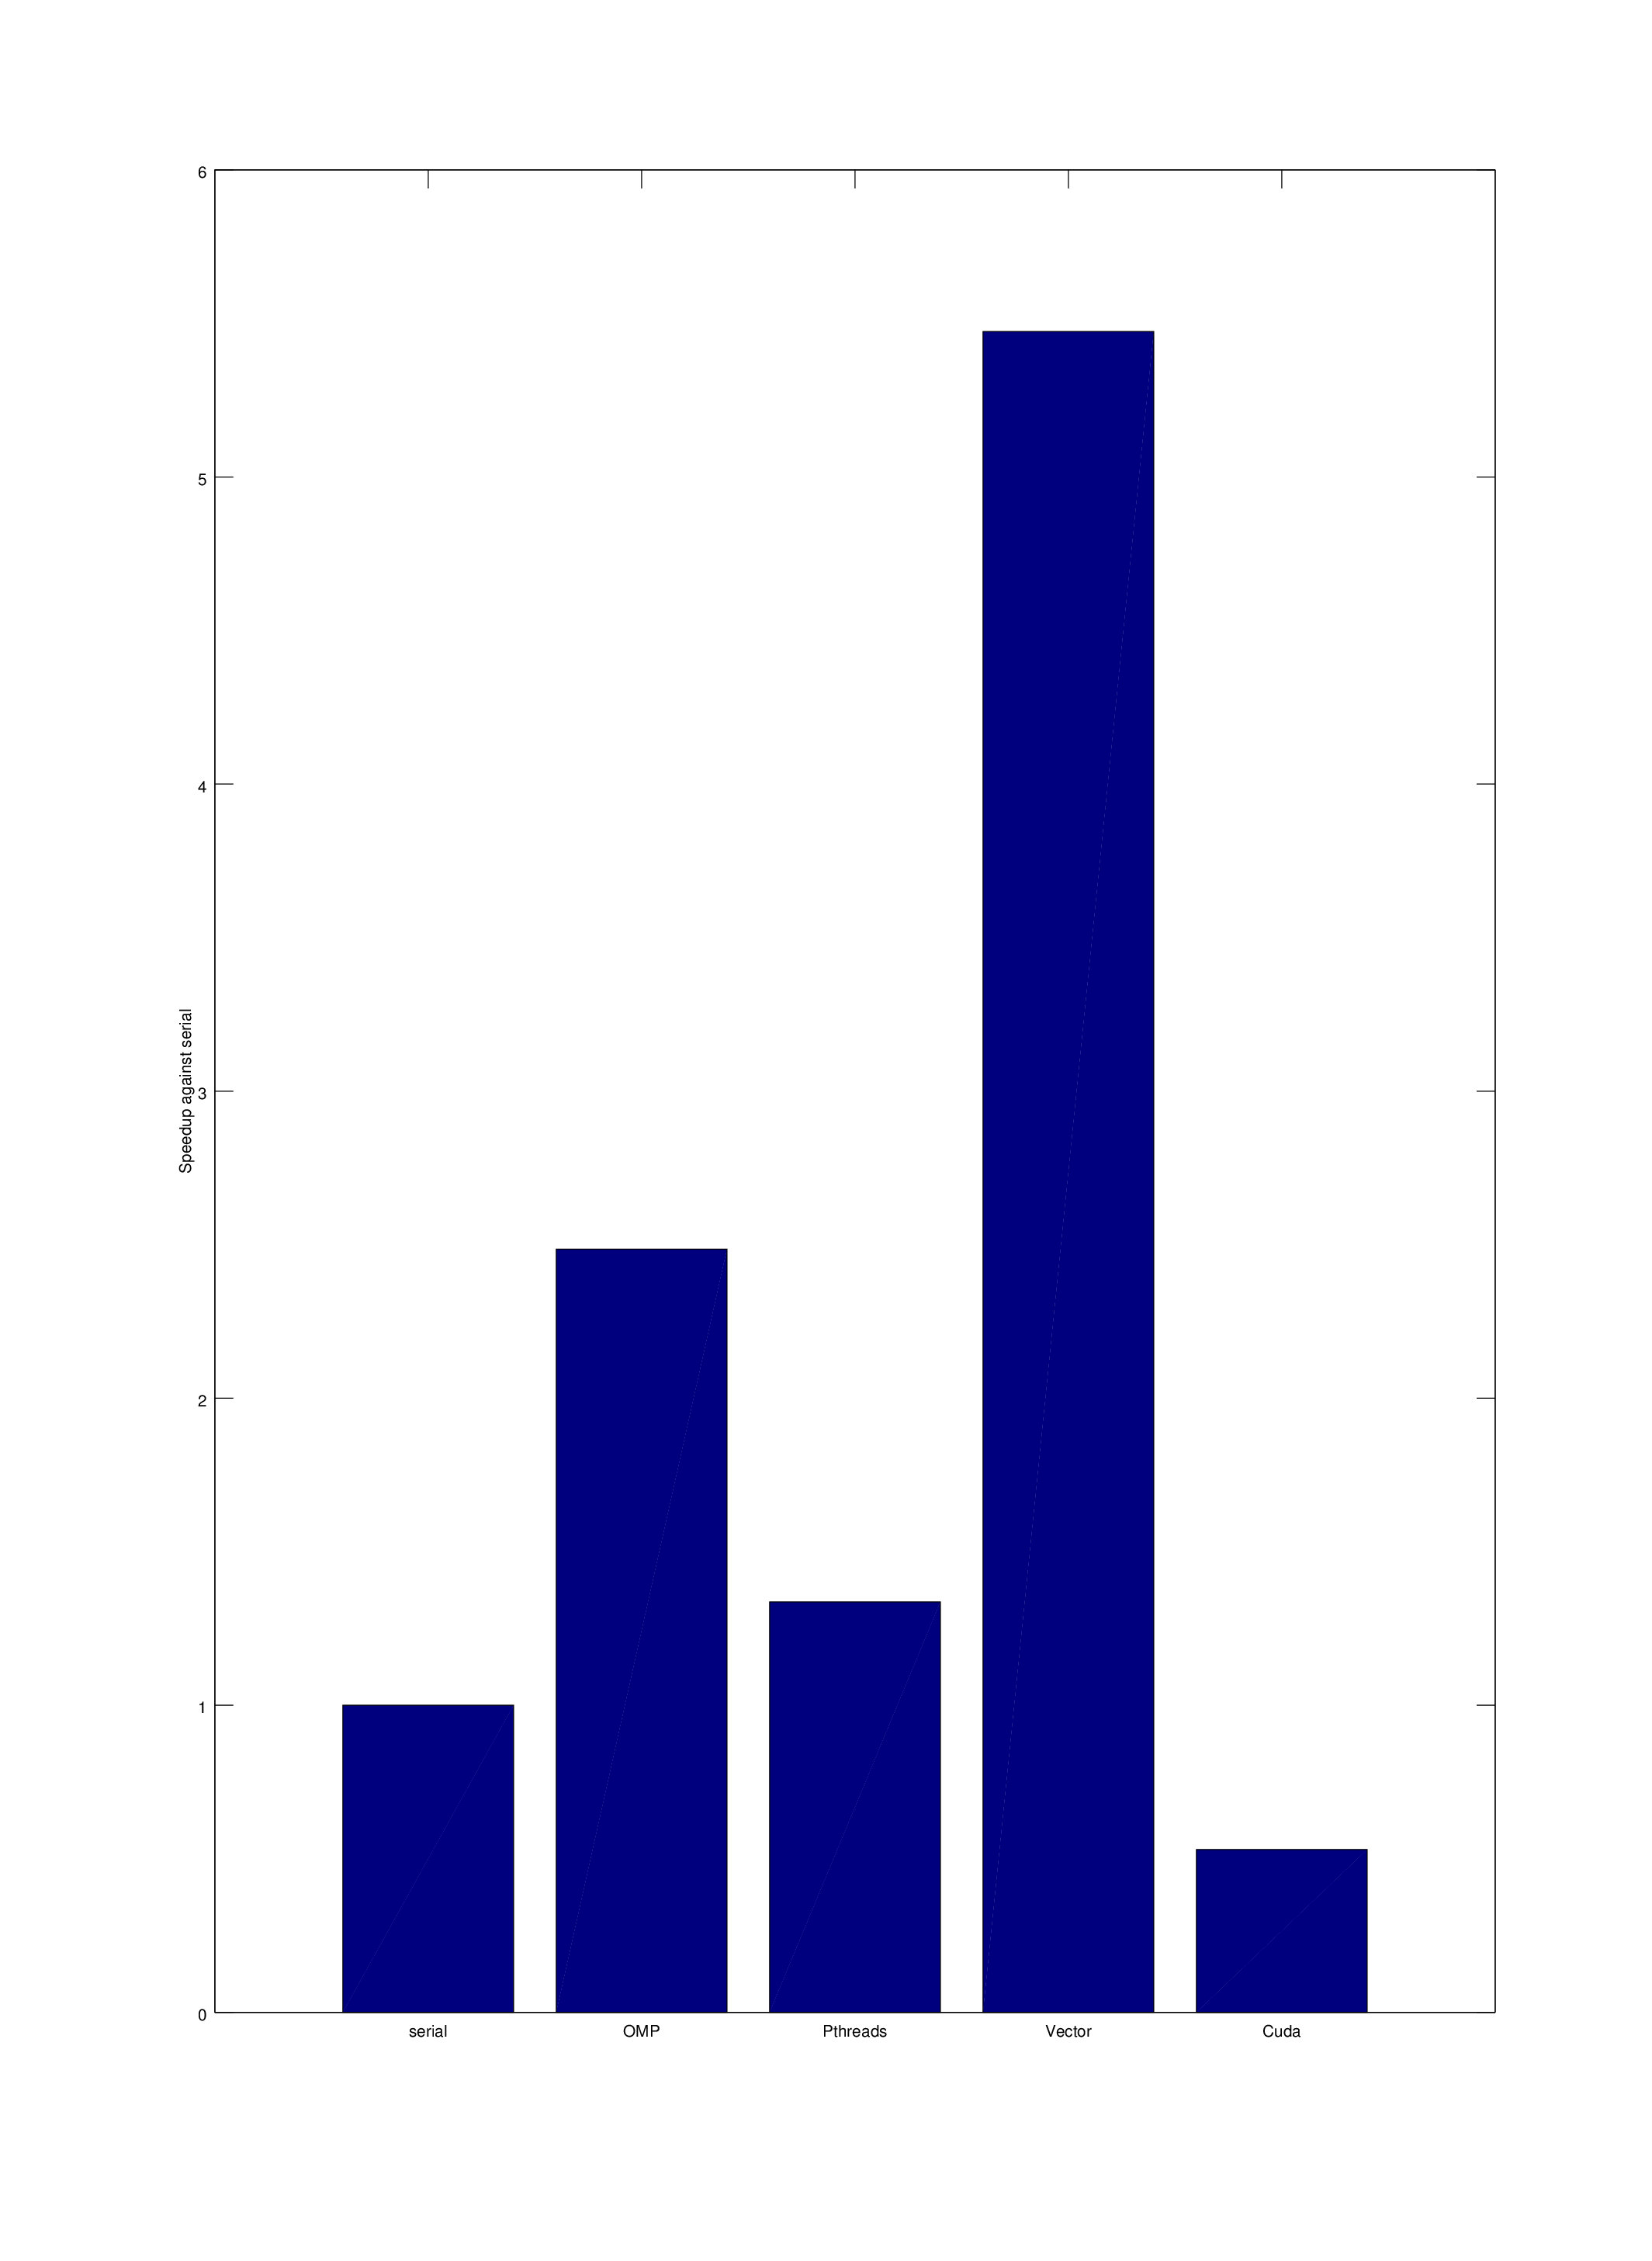
\includegraphics[width=\textwidth]{graph1.png}
\caption{Graph showing the speedup of openmp, pthreads, SIMD and CUDA for a moderately sized scenario with 2048 agents.}
\label{graph1}
\end{figure}

\begin{figure}[h!]
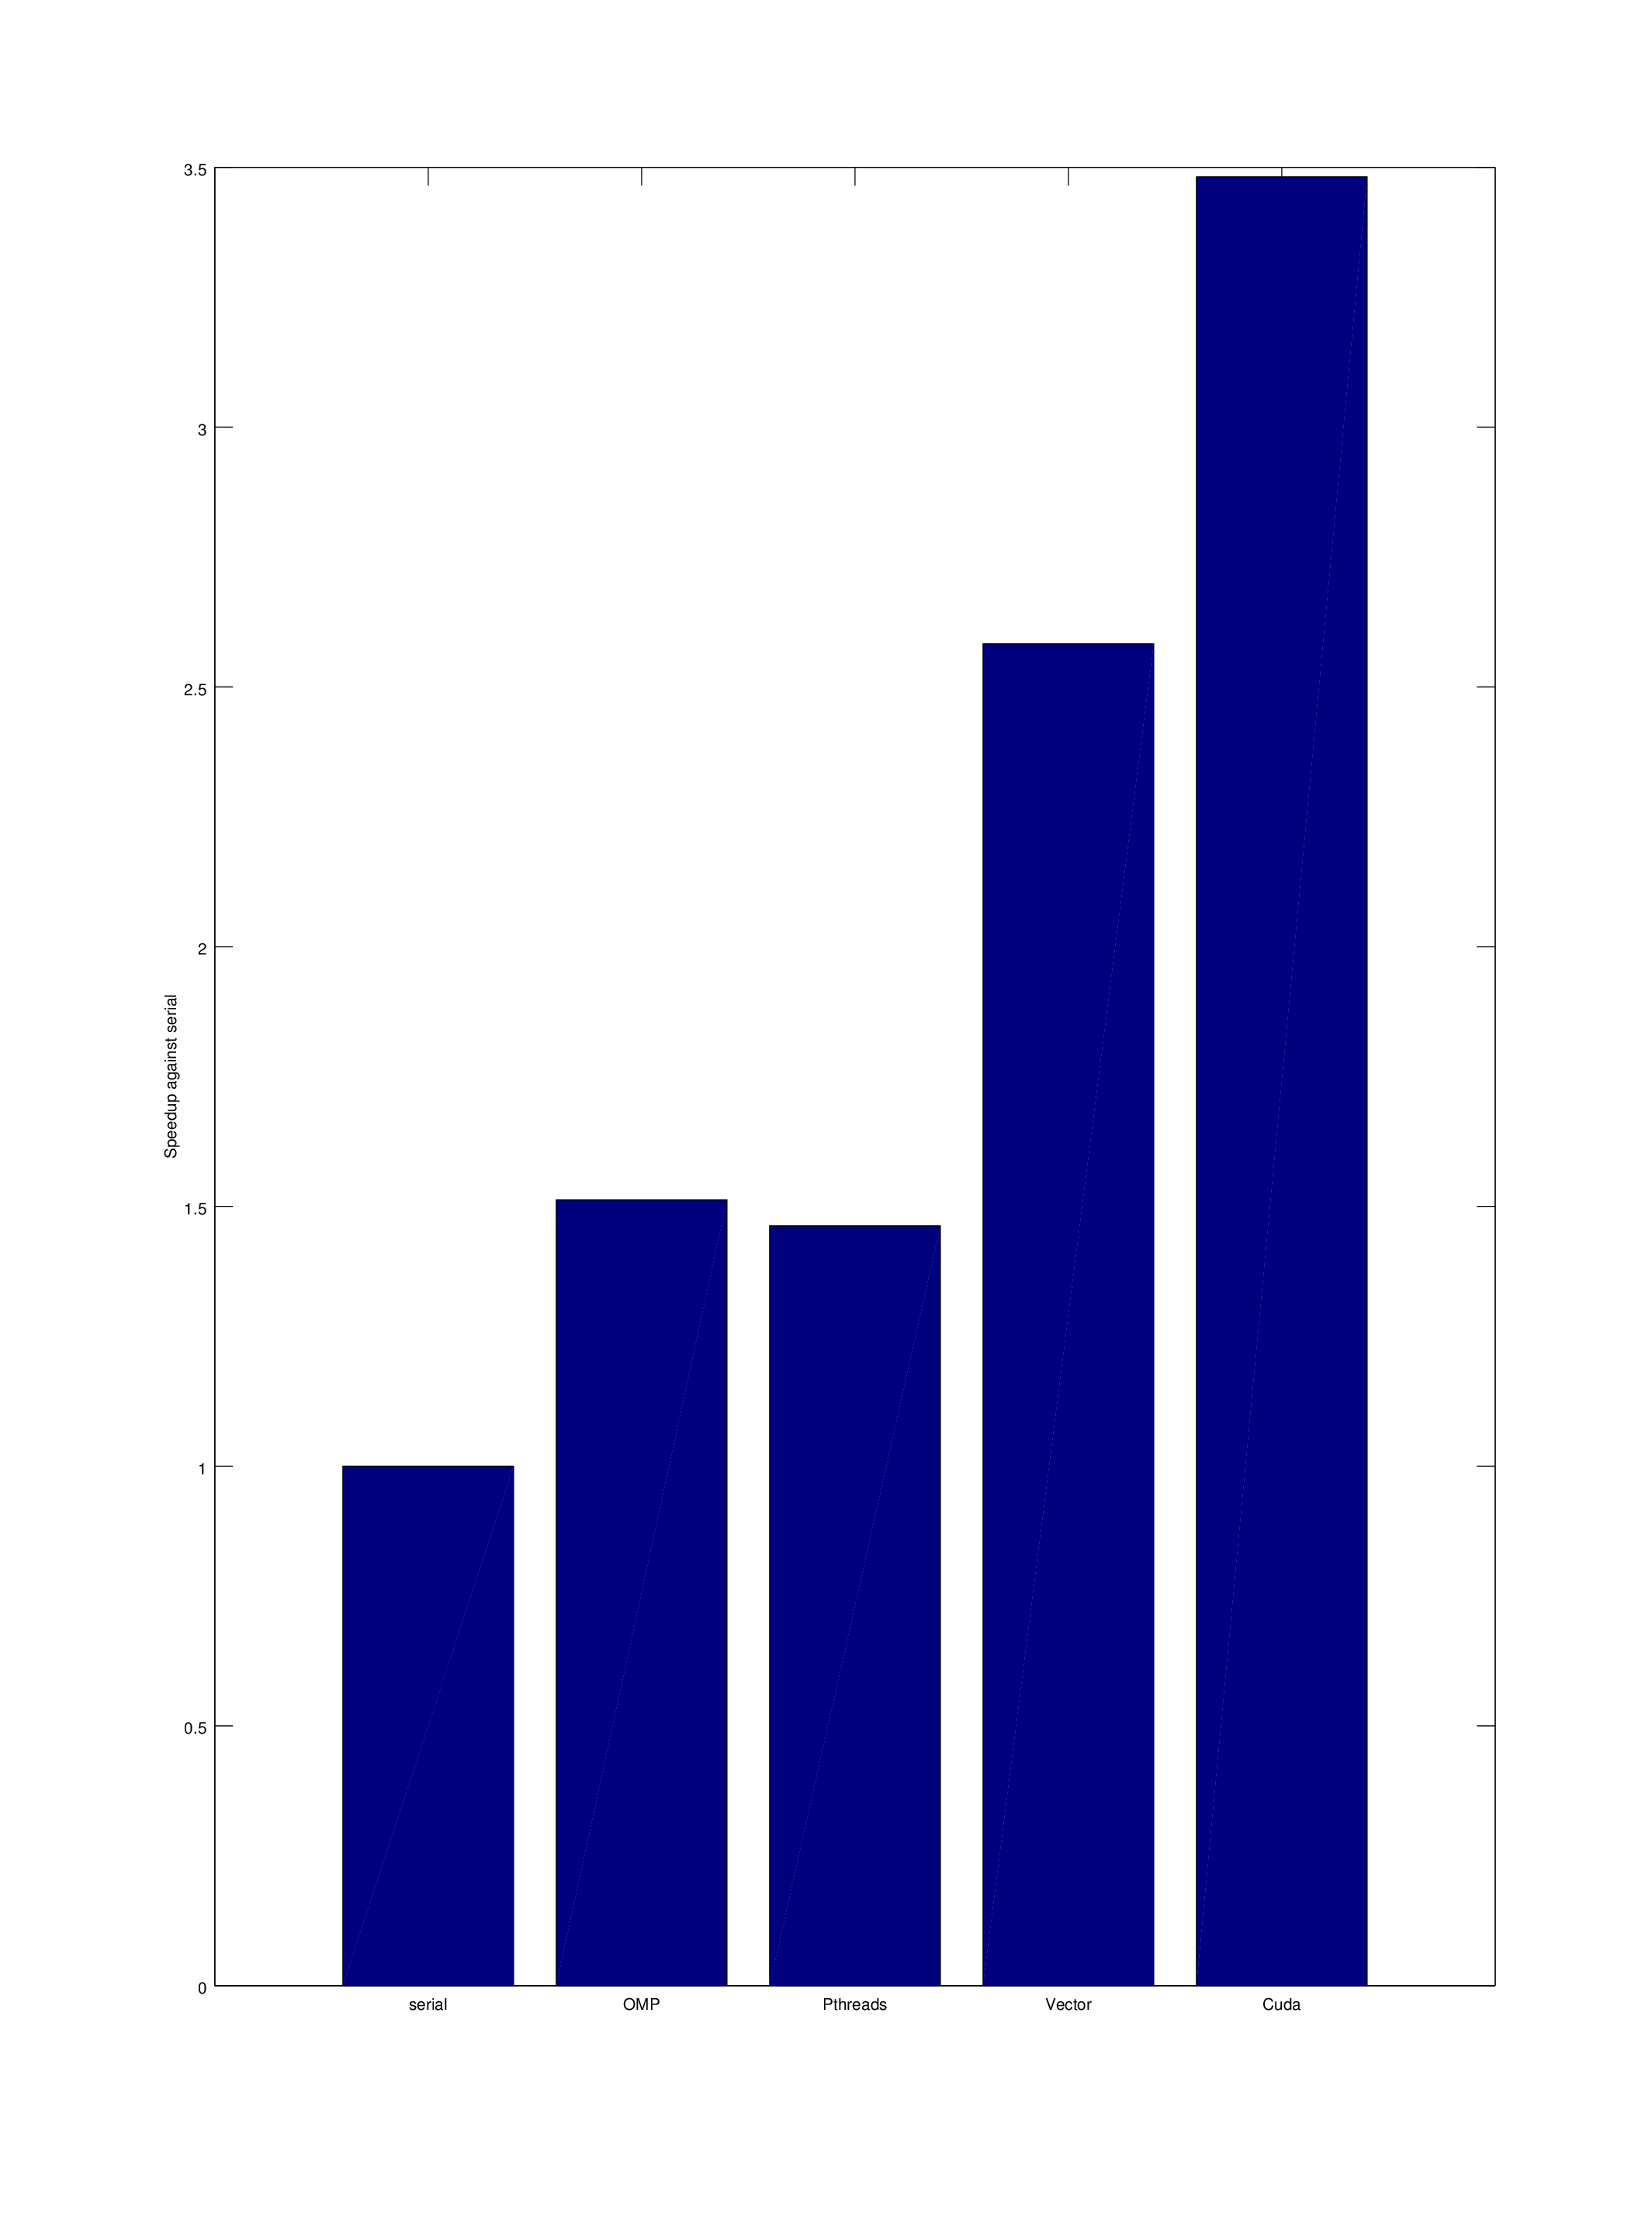
\includegraphics[width=\textwidth]{graph2.png}
\caption{Graph showing the speedup of openmp, pthreads, SIMD and CUDA for a large scenario with 480000 agents.}
\label{graph2}
\end{figure}


\end{document}
